%% Based on a TeXnicCenter-Template by Gyorgy SZEIDL.
%%%%%%%%%%%%%%%%%%%%%%%%%%%%%%%%%%%%%%%%%%%%%%%%%%%%%%%%%%%%%

%------------------------------------------------------------
%
\documentclass[letterpaper,10pt]{article}
%
\usepackage{amsmath}%
\usepackage{amsfonts}%
\usepackage{amssymb}%
\usepackage{graphicx}
%\usepackage{verbatim}
\usepackage{listings}
%-------------------------------------------
\newtheorem{theorem}{Theorem}
\newtheorem{acknowledgement}[theorem]{Acknowledgement}
\newtheorem{algorithm}[theorem]{Algorithm}
\newtheorem{axiom}[theorem]{Axiom}
\newtheorem{case}[theorem]{Case}
\newtheorem{claim}[theorem]{Claim}
\newtheorem{conclusion}[theorem]{Conclusion}
\newtheorem{condition}[theorem]{Condition}
\newtheorem{conjecture}[theorem]{Conjecture}
\newtheorem{corollary}[theorem]{Corollary}
\newtheorem{criterion}[theorem]{Criterion}
\newtheorem{definition}[theorem]{Definition}
\newtheorem{example}[theorem]{Example}
\newtheorem{exercise}[theorem]{Exercise}
\newtheorem{lemma}[theorem]{Lemma}
\newtheorem{notation}[theorem]{Notation}
\newtheorem{problem}[theorem]{Problem}
\newtheorem{proposition}[theorem]{Proposition}
\newtheorem{remark}[theorem]{Remark}
\newtheorem{solution}[theorem]{Solution}
\newtheorem{summary}[theorem]{Summary}
\newenvironment{proof}[1][Proof]{\textbf{#1.} }{\ \rule{0.5em}{0.5em}}

% Construct the basic page sizes
\oddsidemargin  0.0in
\evensidemargin 0.0in
\textwidth      6.5in
\headheight     0.25in
\topmargin      0.0in
\textheight=8.5in

\begin{document}

\title{Using GMAT's C Interface Library\\\large{Revision 0.01, ODTBX Instructions}}
\author{Darrel J. Conway\thanks{Developed under Prime Contract NNG10CP02C, Task Order 28.}
\\Thinking Systems, Inc.}
\date{\today}
\maketitle

\begin{abstract}
This document describes how to use GMAT's C-interface.  It includes descriptions of the methods currently implemented and examples of the calls into the interface made from MATLAB.  It also includes a section showing how to use the interface from ODTBX. 
\end{abstract}

\section{Introduction}

The General Mission Analysis Tool, GMAT, is a space trajectory optimization and mission analysis system developed by NASA and private industry in the spirit of the NASA Vision. GMAT contains new technology and is a testbed for future technology development. One way GMAT provides testbed capabilities is through a library designed to access part of the system's features using calls to C functions.  This document describes that interface.

GMAT is coded in C++ using modern, object oriented design principles.  The implementation of the system in C++ provides challenges for systems written in other languages that want to access GMAT components.  The C interface described here overcomes some of these difficulties by providing simpler calls into GMAT than would be possible if the class structures were accessed directly.  This functionality is limited to the components that have been exposed through the interface.  GMAT's C interface currently provides access to a small subset of the total system, but has been designed to be extended to other components as needed.  The full set of currently implemented elements is provided in Appendix~\ref{sec:FunctionList}.

The following sections describe how to configure a computer to use the C interface, how to make calls into GMAT from MATLAB, and provide an example of the call into GMAT's ODE model for use in an ODTBX integrator.

\section{Setting up the Environment}

GMAT's C interface is implemented as a plugin library that provides access to GMAT objects through C functions.  The library starts a copy of GMAT's engine, loads a configuration by means of a GMAT script, populates a GMAT Sandbox with the configuration, and then provides access to the objects in the Sandbox.

There are several requirements that must be met for the interface to work correctly.  The basic setup procedure can be broken into three pieces: (1)~collecting the files into a set of folders, (2) updating the startup file and configuration script, and (3) testing the setup.

\subsection{Collecting the files}

There are two sets of files that you'll need to organize: those that are found in the folder where you want to run the interface, and the data files GMAT needs to run.  In order to perform the configuration described here, you'll need a functional installation of GMAT on your computer that includes the libCInterface shared library.

The interface needs four files in the run folder - the two shared libraries libGmatBase and libCInterface, the GMAT file gmat\_startup\_file.txt which describes the locations of GMAT's environment data, and the script file defining the configuration of objects that you want to access.  Below I'll describe the steps you take to copy these files into a run folder.  The following steps setup the interface in a folder named InterfaceRunFolder.  Replace that name with the path to the folder you will be using for the interface.  The following instructions describe actions taken from a terminal window (or ``command prompt'' in Windows) for a system with GMT installed in the folder ``/GMAT\_R2011b''; replace that folder name with the path to your installation of GMAT.

\begin{enumerate}
\item If it does not already exist, create the folder in your file system:
\begin{itemize}
\item From a command prompt or console window, type:
\begin{quote}
\texttt{mkdir ~/InterfaceRunFolder} \hfill (Mac or Linux)
\end{quote}
or
\begin{quote}
\texttt{mkdir }\textbackslash\texttt{InterfaceRunFolder} \hfill (Windows)
\end{quote} 
\item Set the current working directory to the new folder:
\begin{quote}
\texttt{cd }\textbackslash\texttt{InterfaceRunFolder}\hfill(Windows)
\end{quote} 
or
\begin{quote}
\texttt{cd ~/InterfaceRunFolder}\hfill(Mac or Linux)
\end{quote} 
\end{itemize}
\item Copy the files needed locally onto the folder:
\begin{itemize}
\item On Windows:
\begin{quote}
\begin{verbatim}
copy \GMAT_R2011b\bin\libGmatBase.dll .
copy \GMAT_R2011b\bin\libCInterface.dll .
copy \GMAT_R2011b\bin\gmat_startup_file.txt .
\end{verbatim}
\end{quote} 
\item On Linux or Mac:
\begin{quote}
\begin{verbatim}
cp /GMAT_R2011b/bin/libGmatBase* .
cp /GMAT_R2011b/bin/libCInterface* .
cp /GMAT_R2011b/bin/gmat_startup_file.txt .
\end{verbatim}
\end{quote} 
\end{itemize}
\end{enumerate}

\noindent You'll also need a script defining the configuration you want to access through the interface.  A sample script is shown in Appendix~\ref{sec:SampleConfigurationScript}.  Place the test for this script in a file named GmatConfig.script.  Once you have finished these instruction, you should have the following files in InterfaceRunFolder:
\begin{itemize}
	\item gmat\_startup\_file.txt
	\item libGmatBase.dll, libGmatBase.so, or libGmatBase.dylib
	\item libCInterface.dll, libCInterface.so, or libCInterface.dylib
	\item GmatConfig.script
\end{itemize}

Finally, if you are planning to access GMAT from MATLAB, your MATLAB environment will need access to the script files that drive the interface.  These files are in the trunk code of the ODTBX project, in the folder trunk{\textbackslash}ODTBX\_Source{\textbackslash}GMAT\_Adapters.  We will add this folder to the MATLAB path below; be sure that you have access to the folder if you are using MATLAB.

\subsection{Updating the configuration file and script}

Appendix~\ref{sec:DataFileOrganization} describes the standard data file organization for GMAT.  This file organization is described in the GMAT startup file, gmat\_startup\_file.txt.  There is no need to move the data files into your interface run folder.  Instead, open the startup file, and look for these lines:

\begin{quote}
\begin{verbatim}
#-----------------------------------------------------------
ROOT_PATH              = ../
#-----------------------------------------------------------
PLUGIN                 = ../plugins/proprietary/libVF13Optimizer
PLUGIN                 = ../plugins/libGmatEstimation
PLUGIN                 = ../plugins/libMatlabInterface
PLUGIN                 = ../plugins/libFminconOptimizer
#-----------------------------------------------------------
OUTPUT_PATH            = ../output/
LOG_FILE               = OUTPUT_PATH/GmatLog.txt
REPORT_FILE            = OUTPUT_PATH/GmatReport.txt
SCREENSHOT_FILE        = OUTPUT_PATH
#-----------------------------------------------------------
MEASUREMENT_PATH       = OUTPUT_PATH/
#-----------------------------------------------------------
EPHEM_PATH             = OUTPUT_PATH/
#-----------------------------------------------------------
#GMAT_FUNCTION_PATH    = 
#-----------------------------------------------------------
#MATLAB_FUNCTION_PATH  = 
#-----------------------------------------------------------
DATA_PATH              = ROOT_PATH/data/
#-----------------------------------------------------------
\end{verbatim}
\end{quote}

Begin by removing the PLUGIN lines or editing them to point to your GMAT folder.  Insert this line at that location:  

\begin{quote}
\begin{verbatim}
PLUGIN                 = libCInterface
\end{verbatim}
\end{quote}

\noindent Change the ROOT\_PATH and the OUTPUT\_PATH entries to the current folder: 

\begin{quote}
\begin{verbatim}
ROOT_PATH              = ./
...
OUTPUT_PATH            = ./
\end{verbatim}
\end{quote}

\noindent Finally, change the DATA\_PATH to point to your GMAT data folder; for instance, 

\begin{quote}
\begin{verbatim}
DATA_PATH              = /GMAT_R2011b/data/
\end{verbatim}
\end{quote}

\noindent The lines listed above should now look like this (with changes to match your configuration): 

\begin{quote}
\begin{verbatim}
#-----------------------------------------------------------
ROOT_PATH              = ./
#-----------------------------------------------------------
PLUGIN                 = libCInterface
#-----------------------------------------------------------
OUTPUT_PATH            = ./
LOG_FILE               = OUTPUT_PATH/GmatLog.txt
REPORT_FILE            = OUTPUT_PATH/GmatReport.txt
SCREENSHOT_FILE        = OUTPUT_PATH
#-----------------------------------------------------------
MEASUREMENT_PATH       = OUTPUT_PATH/
#-----------------------------------------------------------
EPHEM_PATH             = OUTPUT_PATH/
#-----------------------------------------------------------
#GMAT_FUNCTION_PATH    = 
#-----------------------------------------------------------
#MATLAB_FUNCTION_PATH  = 
#-----------------------------------------------------------
DATA_PATH              = /GMAT_R2011b/data/
#-----------------------------------------------------------
\end{verbatim}
\end{quote}


\subsection{Testing the Setup from MATLAB}

At this point, the C interface is ready for testing.  To test the interface from MATLAB, start MATLAB and change your working folder to the interface folder.  Add the path to the GMAT\_Adapters folder from the ODTBX source to your MATLAB environment with this command (on Windows, assuming the ODTBX source code is in the C:{\textbackslash}ODTBX-Trunk folder):

\begin{quote}
\begin{verbatim}
addpath C:\ODTBX-Trunk\ODTBX_Source\GMAT_Adapters
\end{verbatim}
\end{quote}

\noindent or this command (on Mac or Linux, with the ODTBX code in the ~/ODTBX-Trunk folder):

\begin{quote}
\begin{verbatim}
addpath ~/ODTBX-Trunk/ODTBX_Source/GMAT_Adapters
\end{verbatim}
\end{quote}

Test the installation by running the startgmat MATLAB function, passing in the name of your configuration script:

\begin{quote}
\begin{verbatim}
>> startgmat('GmatConfig.script');
\end{verbatim}
\end{quote}

\noindent If the configuration is set correctly, you should see a message reporting that GMAT initialized, ran a mission, and retrieves an ODEModel for use in the interface: 
\begin{quote}
\begin{verbatim}
The Moderator has been initialized
Mission run succeeded!
ODE model is set to DefaultProp_ForceModel
\end{verbatim}
\end{quote}

\noindent Now close the GMAT interface and unload it from memory:

\begin{quote}
\begin{verbatim}
>> closegmat
\end{verbatim}
\end{quote}

\noindent This command should result in the following messages: 

\begin{quote}
\begin{verbatim}
Unloading libCInterface...
Unloaded
\end{verbatim}
\end{quote}

\section{Accessing GMAT Objects from MATLAB}

The \texttt{startgmat} and \texttt{closegmat} functions wrap several calls to GMAT's C interface inside of simpler MATLAB functions.  In this section, we'll examine the raw calls into the interface from MATLAB to illustrate how the interface works.  Appendix~\ref{sec:FunctionList} lists all of the functions in the current implementation of the interface.

\textit{To be completed}

\section{An ODTBX Example: Integrating an Orbit}

\textit{To be completed}

\appendix

\section{\label{sec:DataFileOrganization}Data File Organization}

GMAT requires access to data files organized in a file structure described in the GMAT startup file, gmat\_startup\_file.txt.  That file should be in the working folder from which the interface is accessed.  In a typical setup, the GMAT startup file identifies a root folder, a data file folder, and then uses these tow locations to identify the locations of additional data files needed by GMAT.  A typical startup file contains these lines for the top level folders:

\begin{quote}
\begin{verbatim}
ROOT_PATH              = ../
DATA_PATH              = ROOT_PATH/data/
\end{verbatim}
\end{quote}

\noindent The remaining lines in the file describe the locations of planetary ephemerides, coefficient files for planetary gravity fields, time system data, and other data elements needed when GMAT runs.  A typical file structure for the data files is shown in Figure~\ref{fig:DataFileStrucure}.

\begin{figure}[htb]
\begin{center}
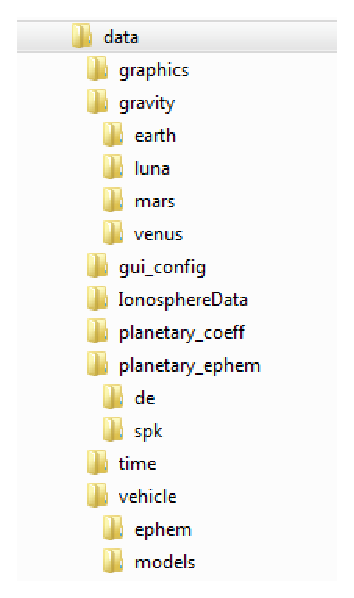
\includegraphics{Images/DataFileLayout.eps}
\caption{The Default Data File Strucure for GMAT}
\label{fig:DataFileStrucure}
\end{center}
\end{figure}

\noindent This file structure matches the structure delivered with GMAT R2011a.  It also matches the data file structure found in the source code repository for GMAT at SourceForge at the time of this writing.  The entries in the GMAT startup file point to specific files in this structure.  For example, the lines

\begin{quote}
\begin{verbatim}
SPK_PATH               = DATA_PATH/planetary_ephem/spk/
PLANETARY_SPK_FILE     = SPK_PATH/de421.bsp
\end{verbatim}
\end{quote}

\noindent identify the location of the SPICE planetary ephemeris file, de421.bsp, in the file system.  Using the entries provided thus far, GMAT looks for the file

\begin{quote}
\begin{verbatim}
../data/planetary_ephem/spk/de421.bsp
\end{verbatim}
\end{quote}

\noindent relative to the starting folder for the system.  The startup file provides similar path data for all of GMAT's data files; interested users should look in this file when trying to understand the data used when running a mission.

\section{\label{sec:FunctionList}Supported Functions}

The C interface supports the following functions:

\begin{quote}
\lstinputlisting{Scripts/CInterfaceFunctions.hpp}
\end{quote} 

\section{\label{sec:SampleConfigurationScript}Sample Configuration Script}

The GMAT engine is configured for use through a GMAT script.  The C-interface specifies this script in the function LoadScript.  Once a script is loaded, it is run and the resulting configuration used by the C interface for further processing.  

A minimal script designed to prepare a point mass gravity model for use by a single spacecraft looks like this:

\begin{quote}
\lstset{numbers=left}
\lstinputlisting{Scripts/defaultConfig.script}
\end{quote}

\noindent The \texttt{PrepareMissionSequence} command on line~34 of this listing tells GMAT to establish all interconnections necessary for the objects in the script, but not to actually exercise these objects.  If you want to actually execute the scripted mission control sequence, use the \texttt{BeginMissionSequence} command here instead.

\end{document}
